\section{Анализ предметной области}
\label{sec:domain}

В данном разделе будет произведен анализ предметной области моделирования пешеходных потоков.

Будет приведена история развития моделей пешеходных потоков, их классификация, достоинства и недостатки некоторых моделей пешеходных потоков.
Также будет произведено сравнение разрабатываемого ПС с существующими аналогами.

\subsection{Модели пешеходных потоков}
\label{sub:domain:models}

\subsubsection{Классификация моделей пешеходных потоков}
\label{sub:domain:models:classification}

Принято классифицировать модели пешеходных потоков по следующим признакам:

\begin{itemize}
  \item По масштабу модели: микроскопические и макроскопические.
        В микроскопической модели можно выделить конкретного пешехода (например, проследить его маршрут).
        В макроскопической модели нельзя выделить отдельного пешехода, объектом моделирования являются пешеходные потоки.
        Примеры микроскопических моделей: модель социальных сил, модель притягивающих сил.
        Пример макроскопической модели: газокинетическая модель.
  \item По дискретности пространства: дискретные и непрерывные.
        Классическим примером дискретной модели является модель на основе клеточного автомата. В данной модели каждый пешеход в один момент времени может занимать только одну клетку, а переход между клетками производится по определенным правилам.
        Примеры непрерывных моделей: газокинетическая модель, модель социальных сил.
  \item По детерминированности: детерминированные и стохастические.
        По причине того, что движение каждого конкретного пешехода зависит от множества различных факторов, моделирование с учетом всех факторов представляется невозможным.
        Хорошей альтернативой является использование стохастических элементов в модели, что позволяет достичь большей реалистичности.
        Большинство моделей включают в себя стохастические элементы, однако есть исключения.
        Наиболее распространенными детерминированными моделями являются расчетные модели "--- набор моделей, относящихся к классу аналитических.
        Данные модели основываются на результатах конкретных опытов и пытаются обобщить их результаты на некоторый класс задач.
\end{itemize}

\subsubsection{История развития моделей пешеходных потоков}
\label{sub:domain:models:history}

Моделирование пешеходных потоков – достаточно новая область в моделировании. Она выделилась из моделирования транспортных потоков в 1980-х годах.
Первоначально для моделирования пешеходных потоков использовались те же подходы, что и для моделирования транспортных потоков.
В это время получила распространение газокинетическая модель.

Газокинетическая модель относится к классу микроскопических моделей, т.е. объектом моделирования является поток людей, без детализации и моделирования каждого конкретного пешехода.
Данный подход хорошо работал для транспортных потоков, однако для пешеходных потоков моделирование каждого конкретного пешехода позволяет достичь более точных результатов.

В связи с этим широкое распространение получили макроскопические модели. Для упрощения расчетов и описания правил использовались дискретные модели, однако вскоре начали появляться и непрерывные модели на основе сил.

\subsubsection{Описание моделей пешеходных потоков}
\label{sub:domain:models:descriptions}

В данном разделе будут приведены описания некоторых моделей пешеходных потоков, а так же их достоинства и недостатки.

\begin{itemize}
  \item Расчетные модели.
        Чаще всего такие модели можно классифицировать как макроскопические, непрерывные и детерминированные.
        Расчетные модели основываются на результатах масштабного эксперимента с участием большого количества людей.
        Результаты эксперимента обрабатываются, и выявляются закономерностей изменения параметров пешеходного потока (его скорость, плотность и т.п.) в зависимости от окружающих условий.
        Затем полученные закономерности можно применять для оценки параметров потока в искомых условиях.
        Преимуществами данного метода можно назвать детерминированность и относительную легкость применения, а недостатком "--- крайней низкую точность полученных результатов.
  \item Газокинетическая модель.
        Макроскопическая, непрерывная, стохастическая модель.
        Использует сходство пешеходных потоков с потоками жидкости/газа, и представляет собой попытку использовать физику термодинамики к пешеходным потокам,
        интерпретируя основные параметры (такие как температура, давление, плотность) по аналогии.
        Позволяет добиться хороших результатов при высоких плотностях пешеходных потоков, что можно отнести к преимуществам данной модели,
        однако показывает очень низкую точность при малых плотностях пешеходных потоков.
  \item Модели на основе клеточного автомата.
        Микроскопические, дискретные модели с возможным элементом стохастичности.
        Пространство представляется в виде сетки.  Каждый пешеход в один момент времени может занимать только одну клетку.
        Движение смоделировано как изменение клеток, где несколько правил применены к пешеходам. Эти наборы правил отличаются в различных реализациях данной модели.
        Чаще всего правила разделяют на два вида: движение к цели и разрешение конфликтов.
        Также могут вводиться дополнительные правила, моделирующие какие-либо внешние условия.
        К преимуществам данной модели можно отнести простоту и скорость работы, а к недостаткам "--- недостаточно реалистичное представление поведения пешехода.
  \item Модель притягивающих сил.
        Микроскопическая, непрерывная, детерминированная модель.
        Представляет пешеходов и препятствия как <<положительно>> заряженные тела, а цели пешеходов "--- как <<отрицательно>> заряженные тела.
        Между каждыми двумя объектами действует аналог кулоновской силы отталкивания либо притяжения.
        Итоговый вектор движения пешехода определяется как сумма всех действующих на пешехода сил.
        Преимущество данной модели "--- простота реализации, а недостаток "--- невозможность расширения модели дополнительными типами поведений.
  \item Модель социальных сил.
        Микроскопическая, непрерывная, стохастическая модель.
        Представляет собой развитие идей, представленных в модели притягивающих сил.
        Основной концепцией в данной модели является абстрактное понятие социальной силы. Под социальной силой понимается мера мотивации пешехода двигаться в определенном направлении.
        Заменяет кулоновские силы притяжения и отталкивания на две отдельных социальных силы: движущую силу (притяжение к цели) и отталкивающую силу (отталкивание от препятствий и других пешеходов).
        Также вводит анизотропность поля зрения и стохастические отклонения от принятого направления.
        Кроме этого, данная модель может быть расширена любой формализованной социальной силой.
        Примерами социальных сил являются сила притяжения к аттракторам (например, аттракторами могут являться информационные знаки), сила объединения пешеходов в группы и многие другие.
        Является самой широко распространенной моделью на текущий момент.
        Позволяет добиться наибольшей реалистичности среди всех рассмотренных моделей, однако платой за это преимущество является скорость работы.
        Чем больше сложных социальных сил введено в модель, тем медленнее она работает.
\end{itemize}

\subsubsection{Выбор модели пешеходных потоков}
\label{sub:domain:models:choice}

Целью данного дипломного проекта является разработка ПС, способного с высокой степенью точности определять вероятные места скопления людей в помещениях.
В соответствии с целью в качестве модели пешеходных потоков в данном курсовом проекте была выбрана модель социальных сил,
так как на данный момент она позволяет добиться наиболее реалистичных результатов.
Ее единственный недостаток "--- низкая скорость работы "--- будет компенсироваться использованием быстрых низкоуровневых языков программирования.

\subsection{Сравнение с аналогами}
\label{sub:domain:analogs}

В данном разделе будет произведено сравнение разрабатываемого ПС с существующими аналогами.

\subsubsection{Pedestrian Dynamics}
\label{sub:domain:analogs:pd}

\newcommand{\iss}{ IN\-CON\-TROL Si\-mu\-la\-ti\-on So\-lu\-ti\-ons }

Pedestrian Dynamics "--- продукт компании \iss.

Компания \iss сотрудничает с нидерландским Утрехтским университетом для построения наиболее реалистичных и эффективных моделей пешеходных потоков.
В качестве модели симуляции Pedestrian Dynamics использует набор сложных эвристических правил, основанных на ряде научных работ.
Также большое внимание уделяется производительности моделирования: используются такие оптимизирующие структуры данных, как сети навигации (navigation mesh) и другие.

В качестве преимуществ использования предложены следующие пункты:
\begin{itemize}
  \item помощь в международной сертификации безопасности сооружений;
  \item обеспечение безопасности использования сооружений;
  \item оптимизация путей эвакуации из сооружения;
  \item быстрое сравнение различных альтернатив с целью выявления лучшего решения;
  \item расчет коммерческой привлекательности определенных областей.
\end{itemize}

Пример результата моделирования можно увидеть на рисунке~\ref{sub:domain:analogs:pd:image_example}.

Компания отмечает следующие преимущества своего продукта:
\begin{itemize}
  \item быстрое и простое построение модели;
  \item поддержка как 2D, так и 3D визуализации;
  \item высокая скорость работы модели;
  \item широкий набор инструментов для построения модели.
\end{itemize}

Пожалуй, единственным недостатком данного продукта является его очень высокая цена.

\begin{figure}[ht!]
  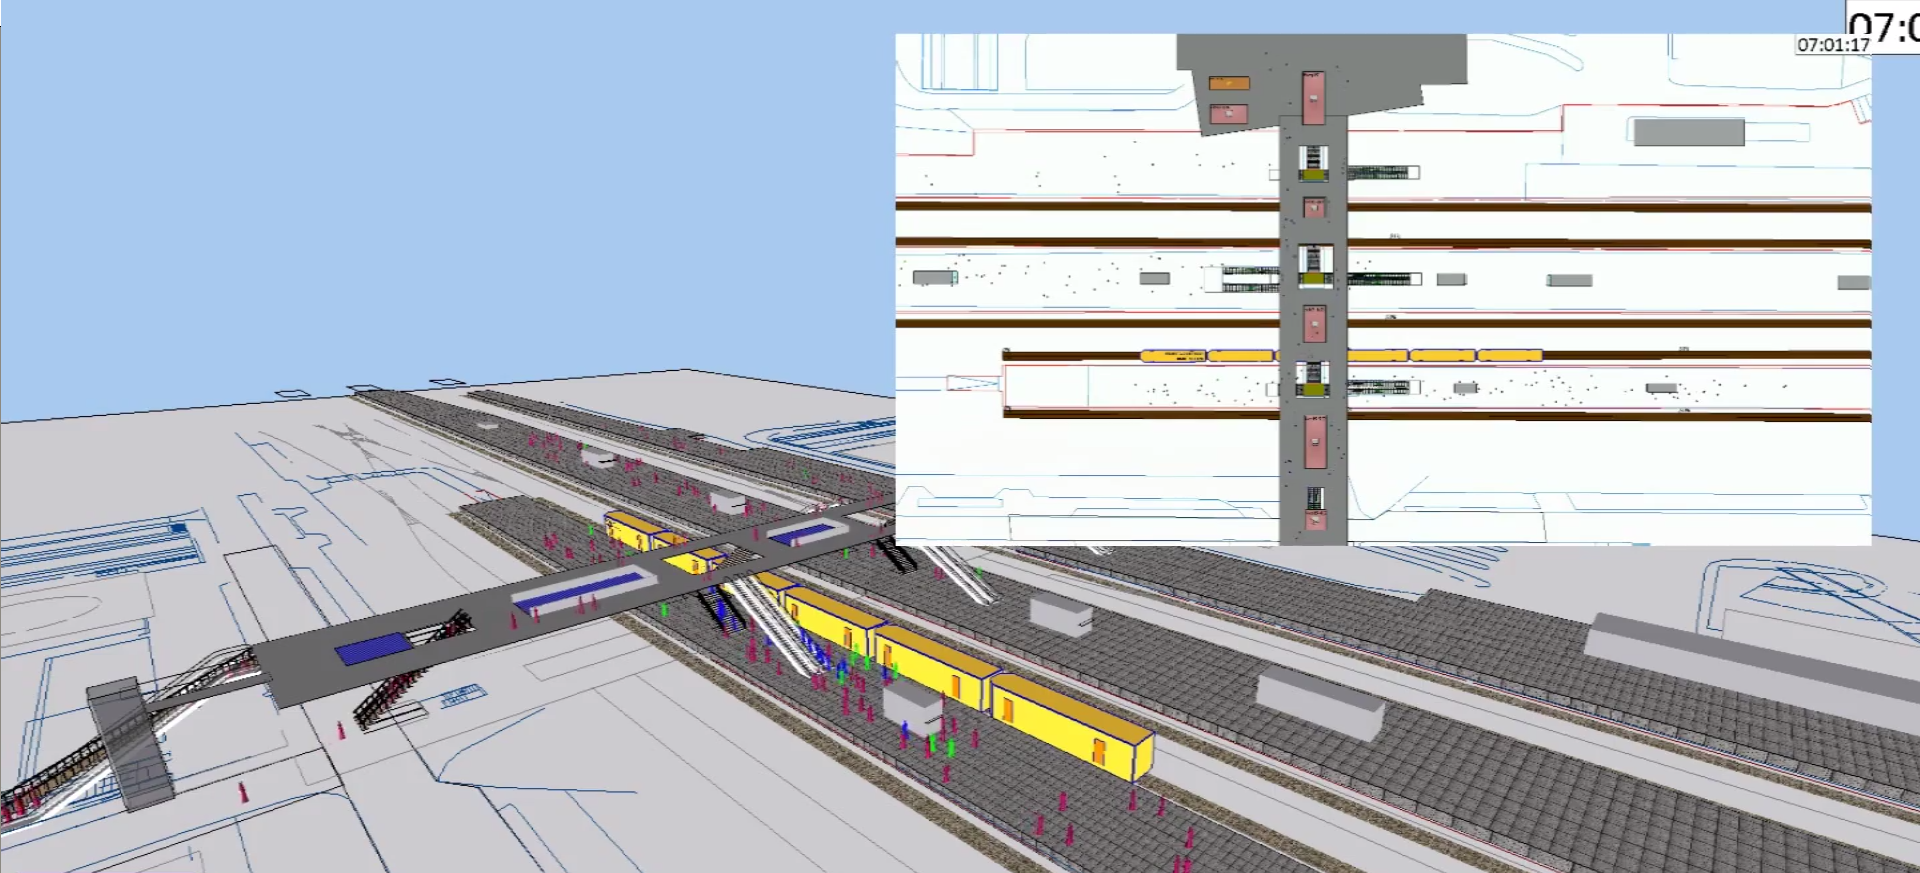
\includegraphics[width=\linewidth]{pedestrian_dynamics}
  \caption{Пример результата моделирования в Pedestrian Dynamics}
  \label{sub:domain:analogs:pd:image_example}
\end{figure}

\subsubsection{Any Logic Pedestrian Flow Module}
\label{sub:domain:analogs:anylogic}

Any Logic \textregistered "--- продукт компании The AnyLogic Company "--- представляет собой набор различных моделей для имитационного моделирования.
В данном разделе будет рассмотрен только один модуль продукта Any Logic \textregistered "--- Any Logic Pedestrian Flow Module.

Возможности Any Logic Pedestrian Flow Module включают в себя следующие пункты:
\begin{itemize}
  \item оценка пропускной способности зданий и отдельных объектов внутри них;
  \item нахождение <<узких мест>> для пешеходных потоков;
  \item оптимизация бизнес-процессов в пунктах обслуживания;
  \item создание и обоснование планов эвакуации при чрезвычайных ситуациях;
  \item оценка плотности потока посетителей торговых зон;
  \item оценка доступности парковок, дорожной сети и общественного транспорта.
\end{itemize}

Пример результата моделирования можно увидеть на рисунке~\ref{sub:domain:analogs:anylogic:image_example}.

К преимуществам данного продукта можно отнести:
\begin{itemize}
  \item Поддержка 2D и 3D визуализации;
  \item Гибкость в выборе и настройки используемой модели;
  \item Широкий набор инструментов для построения модели;
  \item Возможность интеграции моделирования в существующие приложения посредством API.
\end{itemize}

Однако, данный продукт имеет и недостатки:
\begin{itemize}
  \item Низкая скорость работы моделей. Основным языком программирования Any Logic \textregistered является язык программирования Java, что накладывает определенные ограничения на эффективность работы.
  \item Относительная сложность разработки модели.
\end{itemize}

\begin{figure}[ht!]
  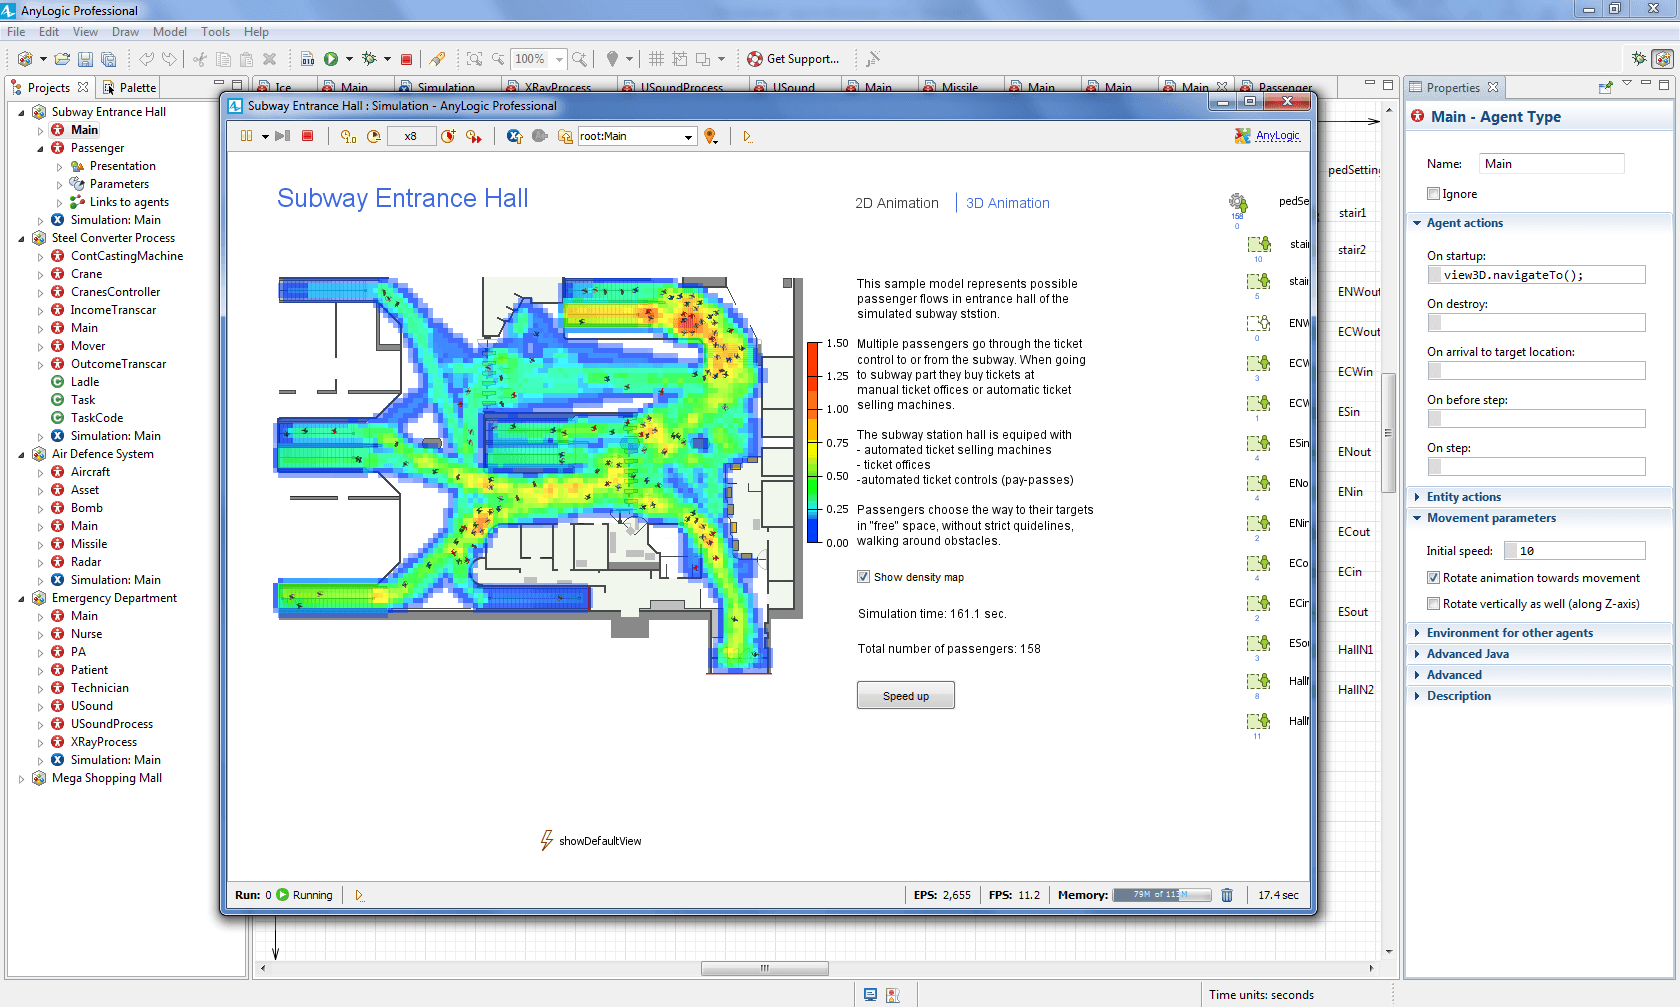
\includegraphics[width=\linewidth]{anylogic}
  \caption{Пример результата моделирования в Any Logic Pedestrian Flow Module}
  \label{sub:domain:analogs:anylogic:image_example}
\end{figure}

\subsubsection{Выводы}
\label{sub:domain:analogs:results}

В результате анализа преимуществ и недостатков продуктов Pedestrian Dynamics и Any Logic \textregistered было решено реализовать ПС, совмещающее в себе преимущества обоих рассмотренных аналогов.
Таком образом, разрабатываемое ПС должно позволять гибко настраивать модель и сценарий симуляции, иметь возможность интеграции моделирования в существующие приложения, но при этом иметь высокую скорость работы.
Более детально требования к разрабатываемому ПС будут рассмотрены в следующем разделе.

\subsection{Требования к разрабатываемому ПС}
\label{sub:domain:requirements}

\subsubsection{Назначение разрабатываемого ПС}
\label{sub:domain:requirements:purpose}

Разрабатываемое ПС должно использоваться при проектировании различных сооружений (вокзалов, станций метро, торговых центров, стадионов) в целях проверки сооружения на наличие потенциально опасных мест скопления людей, а так же для определения максимально допустимого потока пешеходов через данное сооружение.

\subsubsection{Основные выполняемые функции разрабатываемого ПС}
\label{sub:domain:requirements:purpose}

Основной выполняемой функцией разрабатываемого ПС является поиск вероятных областей скопления людей в помещениях.

\subsubsection{Входные данные разрабатываемого ПС}
\label{sub:domain:requirements:purpose}

Входными данными разрабатываемого ПС являются схема исследуемого сооружения и сценарий симуляции.
Более подробно формат схемы и сценария будет описан в разделе <<Проектирование программного средства>>.

\subsubsection{Выходные данные разрабатываемого ПС}
\label{sub:domain:requirements:purpose}

Выходными данными разрабатываемого ПС является 2D анимация пешеходных потоков через исследуемое сооружение с отмеченными вероятными областями скопления людей.

\subsubsection{Дополнительные требования к разрабатываемому ПС}
\label{sub:domain:requirements:purpose}

Разрабатываемое ПС должно удовлетворять следующим требованиям:
\begin{itemize}
  \item Гибкая настройка модели и сценария симуляции.
        Большинство значимых параметров модели и сценария должны быть изменяемыми из файла описания сценария симуляции.
  \item Наличие возможности интеграции моделирования в существующее приложение.
        Результаты моделирования должны быть представлены в простом унифицированном формате.
        Сторонние приложения могут импортировать результаты симуляции и выполнять над ними определенные действия.
  \item Высокая скорость работы.
        Разрабатываемое приложение должно обеспечивать возможность просмотра результатов симуляции в режиме realtime для как минимум одной тысячи пешеходов.
\end{itemize}

\subsubsection{Обоснование выбора языка и средств разработки}
\label{sub:domain:requirements:purpose}

Разрабатываемое ПС можно разбить на три модуля:
\begin{itemize}
  \item модуль чтения и разбора схемы сооружения и сценария симуляции;
  \item модуль выполнения симуляции;
  \item модуль отображения результатов симуляции в виде 2D анимации.
\end{itemize}

К каждому из этих модулей предъявляются свои требования по производительности и надежности, поэтому было решено использовать разные языки программирования для каждого модуля.

Модуль чтения и разбора схемы сооружения и сценария симуляции не требователен к производительности, поэтому для него было решено использовать язык Ruby.
Также выбор языка Ruby позволяет оформить сценарий симуляции в виде DSL (Domain Specific Language "--- предметно"=ориентированный язык) за счет удобной реализации метапрограммирования в Ruby.

Модуль выполнения симуляции "--- самый важный модуль в разрабатываемом ПС. К нему предъявляются высокие требования как по производительности, так и по надежности.
Идеальным выбором в данном случае является язык программирования Rust. Rust является низкоуровневым языком, что позволяет писать на нем высокоэффективные приложения.
Также Rust поддерживает проверку безопасности и в некоторых случаях корректности кода во время компиляции.
Это улучшает безопасность разрабатываемого ПО, а так же позволяет не вводить такие проверки во время выполнения программы, что позволяет увеличить эффективность.

Модуль отображения результатов симуляции в виде 2D анимации не столь требователен к производительности и надежности.
Выбор языка программирования С++ для него обусловлен наличием для С++ удобной библиотеки векторной анимации SDL.
